\documentclass[review]{elsarticle}
\usepackage{lineno,hyperref,amssymb,graphicx,booktabs}

\modulolinenumbers[5]
\journal{Nuclear Instruments and Methods in Physics Research A}


% Note from Jeff: Our previous NMOR article was 20 pages in this
% format, which became about 6 pages in the final paper in NIMA.


%%%%%%%%%%%%%%%%%%%%%%%
%% Elsevier bibliography styles
%%%%%%%%%%%%%%%%%%%%%%%
%% To change the style, put a % in front of the second line of the current style and
%% remove the % from the second line of the style you would like to use.
%%%%%%%%%%%%%%%%%%%%%%%

%% Numbered
%\bibliographystyle{model1-num-names}

%% Numbered without titles
%\bibliographystyle{model1a-num-names}

%% Harvard
%\bibliographystyle{model2-names.bst}\biboptions{authoryear}

%% Vancouver numbered
%\usepackage{numcompress}\bibliographystyle{model3-num-names}

%% Vancouver name/year
%\usepackage{numcompress}\bibliographystyle{model4-names}\biboptions{authoryear}

%% APA style
%\bibliographystyle{model5-names}\biboptions{authoryear}

%% AMA style
%\usepackage{numcompress}\bibliographystyle{model6-num-names}

%% `Elsevier LaTeX' style
%\bibliographystyle{elsarticle-num}
%%%%%%%%%%%%%%%%%%%%%%%

\begin{document}

\begin{frontmatter}

\title{Sensitivity of Fields within Magnetically Shielded Volumes to
  Changes in Permeability}

\author[manitoba]{T. Andalib\corref{mycorrespondingauthor}}
\cortext[mycorrespondingauthor]{Corresponding author}
\ead{andalibt@myumanitoba.ca}
\author[winnipeg,manitoba]{C.P. Bidinosti}
\author[winnipeg,manitoba]{R.R. Mammei}
\author[winnipeg,manitoba]{J.W. Martin}
\author[winnipeg]{D. Ostapchuk}

\address[winnipeg]{Physics Department, The University of Winnipeg, 515 Portage Avenue, Winnipeg, MB, R3B 2E9, Canada}
\address[manitoba]{Department of Physics and Astronomy, University of Manitoba, Winnipeg, MB R3T 2N2, Canada}


\begin{abstract}
Future experiments seeking to measure the neutron electric dipole
moment (nEDM) require stable and homogeneous magnetic fields.  The
stability of the magnetic field within a magnetically shielded volume
is influenced by a number of factors.  In this paper, we study one of
these factors, which is the dependence of the internally generated
field on the permeability of the material.  We also provide
measurements of the temperature-dependence of the permeability of the
material, and indicate the extrapolation yet required to adequately
use these measurements to design future nEDM experiments.
\end{abstract}

\begin{keyword}
Magnetic Shielding \sep Neutron Electric Dipole Moment \sep Magnetic Field Stability
\end{keyword}

\end{frontmatter}

\linenumbers

\section{Introduction}

The next generation of neutron electric dipole moment (EDM)
experiments aim to measure the EDM $d_n$ with proposed precision
$\delta d_n\lesssim
10^{-27}$~e-cm~\cite{bib:nedm1,bib:nedm2,bib:nedm2.5,bib:nedm3,bib:nedm3.5,bib:nedm4,bib:nedm5,bib:nedm6,bib:nedm6.5}.
In the previous best experiment \cite{bib:pendlebury}, which discovered
$d_n<3\times 10^{-26}$~e-cm (90\% C.L), effects related to magnetic field
homogeneity and instability were found to dominate the systematic
error.  A detailed understanding of passive and active magnetic
shielding, magnetic field generation within shielded volumes, and
precision magnetometry is expected to be crucial to achieve the
systematic error goals for the next generation of experiments.  Much
of the R\&D effort for these experiments is focused on careful design
and testing of various magnetic shield geometries with precision
magnetometers~\cite{bib:brys,bib:afach,bib:fierlingerroom,bib:sturmthesis,bib:patton}.

%\begin{itemize}
%\item General requirements on field, stability of field, stability of gradient.
%\item List all possible factors that can affect field stability -
 % degaussing, vibrations, etc. possibly with additional references.
%\item State the problem addressed in this paper (changes in $\mu$) and
 % the result.
%\end{itemize}
The nEDM experiment at TRIUMF aims to determine $\delta d_n \sim
10^{-27}$ e$\cdot$cm. This level of precision requires a 1 $\mu$T
magnetic field with the homogeneity of $<$ 1 nT/m and the stability of
pT over the UCN free-precession time.

%%%%%%%%%%%%%%%%%%%%%%%%%%%%%%%%%%%%%%%%%%%%%%%%%%%%%%%%%%%%%%%%%%%%
% Taraneh
%%%%%%%%%%%%%%%%%%%%%%%%%%%%%%%%%%%%%%%%%%%%%%%%%%%%%%%%%%%%%%%%%%%%
% 
% general layout of magnetic system for an EDM experiment
%

The magnetic field system for the future nEDM experiment at TRIUMF comprises the components used to null environment magnetic fields and provide a stable homogeneous static magnetic field. It includes an active compensation system, a magnetically shielded room (MSR), several more layers of passive shielding, and  an internal coil system.
The active compensation system will be used to reduce the external magnetic field at the measurement site to $\mu$T level and prevent the saturation of the passive magnetic shields.
The passive shielding system nullifies the residual background fields to the pT level with a two-stage system including a 2-layer MSR and a smaller 3-layer shield that fits inside the room and surrounds the nEDM apparatus.
Mechanical and temperature changes of this system and the demagnetization procedure of the passive magnetic shielding will affect the stability of the magnetic field within the measurement volume\cite{bib:thiel,bib:altarev2014,bib:altarev2015,bib:voigt}.

%
% demagnetization:  cite Thiel et al., recent Fierlinger paper
%

%
% mech/temp:  cite BMSR paper
%

%
% mech - other citations?  What have other people done to characterize
% their MSR's?
%


The passive shields for the nEDM experiments are made of highly
permeable materials such as Mu-Metal which is an Ni-Fe alloy that
allows measurements at low frequency magnetic fields. These alloys
operate at room temperature and are sensitive to small temperature
variations which affects the electromagnetic behaviour of the material
such as the magnetic permeability, $\mu$ \cite{bib:couderchon,bib:kruppvdm}. For
these type of alloys $\mu$ depends also on the annealing process
\cite{bib:gupta,bib:bozorth}. 



%The temperature dependence of $\mu$ has been measured from two different approaches and the overall result found to be 0.1\%/K $<\frac{1}{\mu} \frac{d\mu}{dT}<$2.3\%/K.

%%%%%%%%%%%%%%%%%%%%%%%%%%%%%%%%%%%%%%%%%%%%%%%%%%%%%%%%%%%%%%%%%%%%
% Taraneh
%%%%%%%%%%%%%%%%%%%%%%%%%%%%%%%%%%%%%%%%%%%%%%%%%%%%%%%%%%%%%%%%%%%%
% 
% more literature?
%


\section{Sensitivity of Internally Generated Field to Permeability of the Shield $B_0(\mu)$}

\subsection{Analytical Calculations in Spherical (and Cylindrical) Geometry}

%%%%%%%%%%%%%%%%%%%%%%%%%%%%%%%%%%%%%%%%%%%%%%%%%%%%%%%%%%%%%%%%%%%%55
% Taraneh
%%%%%%%%%%%%%%%%%%%%%%%%%%%%%%%%%%%%%%%%%%%%%%%%%%%%%%%%%%%%%%%%%%%%55
%\begin{itemize}
%\item State basic physics of problem, define reaction factor, note
%  return flux through shield, etc.
%\item State formulae and results for reasonable parameters.
%\item Possibly one graph of $B_0(\mu)$ with both geometries.
%\end{itemize}

The presence of a coil inside the innermost passive shield turns the
shield into a return yoke and it is due to the penetration of the
magnetic field flux into the magnetic shield. The ratio of the
magnetic field inside the coil in the presence of the magnetic shield
to the coil in free space can be called the reaction factor $C$ which
is $>$ 1 for spherical and cylindrical
geometries~\cite{bib:bidinosti}. The coupling of the coil to the
innermost layer of the magnetic shield suggests that any changes in
the properties of the magnetic shield gives rise to a change in the
internal field. One of these properties is $\mu$ which is of
significant importance because of the high permeability of the passive
shields. As a result, the stability of the magnetic shields
contributes to the stability of the internal field.

%From Refs. \cite{bib:smythe, bib:ferraro} for a zonal surface current
%\begin{equation}
%\bold{F}=- \sum_{n=1} ^{\infty} \frac{C_n}{\ell} P^1 _n (u) \hat{\phi}
%\end{equation}
%bound on a sphere with radius $\ell$ the magnetic field at $r < \ell$ and $r>\ell$ is calculated.
%The case of an ideal spherical surface current ($n=1$) inside a spherical shell with inner radius $a$ and outer radius $b$ has been analytically calculated considering the following boundary conditions

%\begin{equation}
%\frac{1}{\mu_0} B_{\theta} (a^-) = \frac{1}{\mu} B_{\theta}(a^+)
%\end{equation}
%\begin{equation}
%\frac{1}{\mu}B_{\theta}(b^-)=\frac{1}{\mu_0}B_{\theta}(b^+).
%\end{equation}
%Fig. \ref{fig:Magnetic_Field} shows the magnetic field $B$ as a function of relative $\mu$ for $\ell=0.53$ m, $a=0.57$ m and a thickness of 1.5 mm for the shield which are comparable to the dimensions of the ILL nEDM experiment setup \cite{bib:baker, bib:knecht}.

%%%%%%%%%%%%%%%%%%%%%%%%%%%%%%%%%%%%%%%%%%%%%%%%%%%%%%%%%%%%%%%%%%%%55
% Taraneh
%%%%%%%%%%%%%%%%%%%%%%%%%%%%%%%%%%%%%%%%%%%%%%%%%%%%%%%%%%%%%%%%%%%%55
% make it clear this is for a spherical geometry that is close to the
%  ILL geometry.
%
Fig.~\ref{fig:Magnetic_Field} shows the central magnetic field $B$ as
a function of relative $\mu_r=\mu/\mu_0$ for coil radius 0.53~m inside
a magnetic shield with the inner radius of $0.57$~m and a thickness of
1.5~mm which are comparable to the dimensions of the ILL nEDM
experiment geometry~\cite{bib:baker,bib:knecht}.
\begin{figure}[h!]
\begin{center}
   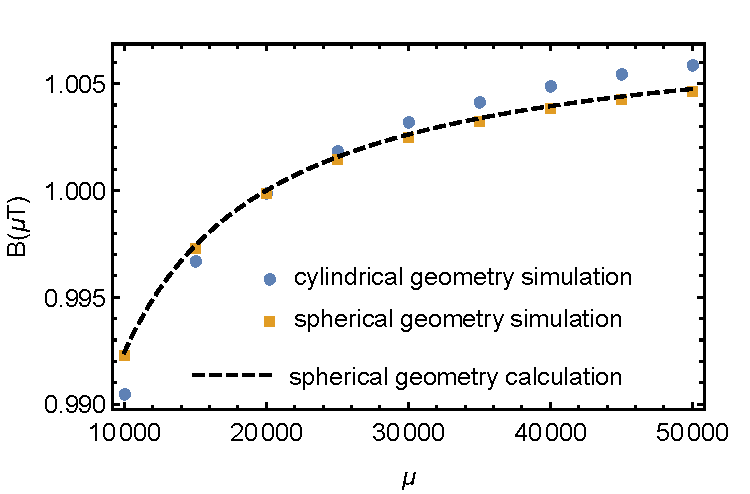
\includegraphics[width=0.6\textwidth]{femm_and_calcs.pdf}
    \caption{Magnetic field as a function of relative magnetic
      permeability $\mu_r$ for geometries similar to the ILL nEDM
      experiment.  The dashed line is for an ideal spherical surface
      current of radius $0.53$~m inside a spherical shell of inner
      radius 0.57~m, thickness 1.5~mm.  Open and close circles are
      FEMM-based simulations of spherical and cylindrical geometries
      with similar dimensions, described in the text.  The coil
      currents have been arranged to give a $1~\mu$T field at the
      $\mu_r=20000$ point.}
    \label{fig:Magnetic_Field}
    \end{center}
\end{figure} 
For a 10\% change in relative $\mu$ (from 20000 to 22000), the
magnetic field changes by 0.7~nT.



\subsection{Magnetostatic Simulation Results \label{sec:femm}}

Finite-element analysis simulations were conducted to analyze the
effect of discretizing the surface current, and to test the geometry
dependence of the sensitivity of the experiment to changes in $\mu$.
Two axially symmetric simulations were conducted using
FEMM~\cite{bib:femm}.  In the first simulation, the same spherical geometry was
used as for the analytical calculations.  However, the surface current
was discretized to 50 individual circular wire, inscribed onto a
sphere, and equally spaced vertically (i.e.~a discrete sin$\phi$
coil).  A square coil profile of side length 1~mm was used.  As shown
in Fig.~\ref{fig:Magnetic_Field}, this simulation gave good agreement
with the analytical calculation.

As an example of one additional axially symmetric geometry, a solenoid
within a cylindrical shield was simulated, with equal coil spacings.
In the limit of infinite $\mu$, the image currents in the end caps of
the shield are an infinite series of coils, giving an ideal infinite
solenoid with a uniform field.  Again, fifty discrete coils were
simulated, where the spacing from an end coil to the inner face of the
shield end-cap being half the inter-coil spacing, as appropriate to
generate the correct image currents in the infinite $\mu$ limit. 

As shown in Fig.~\ref{fig:Magnetic_Field}, the slope of $B(\mu)$ is
somewhat steeper, and similar in magnitude to the spherical case.  We
therefore conclude that the scale of the sensitivity of a generic nEDM
experiment to global changes in the magnetic permeability is
$\frac{\mu}{B}\frac{dB}{d\mu}\sim 0.01$.

In the spherical case the reaction factor is 1.39, meaning that the
field generated by the spherical coil is amplified by this
multiplicative factor by the presence of the magnetic shield (flux
return).  In the cylindrical case the reaction factor is 1.35.  If the
reaction factor is closer to unity, the calculated
$\frac{\mu}{B}\frac{dB}{d\mu}$ will be smaller, and the EDM experiment
less sensitive to changes in $\mu$.  The results in the two geometries
show that there is also a weaker geometry-dependence to this
statement.


%\begin{itemize}
%\item I think it would be easy to provide results in axisymmetric
%  geometries from FEMM.
%\item If any result is available from OPERA, it could be included here.
%\item Results should be for a restricted set of possible nEDM coils.
%\item quote reaction factors?
%\item One graph?  % probably the same graph as above
%\end{itemize}

\subsubsection{Field within the passive flux return for EDM experiments}
The total magnetic flux produced by the coil is conserved. It means,
the total number of the magnetic field lines that come out of the coil
will enter the shield material. Therefore the magnetic field internal
to the material can be estimated. For a cylindrical geometry similar
to what described in Sec. \ref{sec:femm}, the $B$ field is 170
$\mu$T. At $\mu$=20000, the $H$ field would be 0.007~A/m.

% Taraneh to do: state B, H in the material arising from these
% simulations.  (It can be calculated in FEMM very easily, and will
% agree perfectly with analytical calculation.  Perhaps we should just
% look it up in the FEMM simulation.)

% State principle of conservation of flux, useful for analytical
% calculations.

% Note that the value is therefore very weakly dependendent on mu.

% Jeff to do: this is not enough information and needs to be edited
% and likely increased.  Need to create a task list and gather more
% numbers.

\subsection{Self-Shielded Coils}

A way to decouple the internal coil from the magnetic shield is to
design a self-shielded
coil~\cite{bib:cpviolwithoutstrangeness,bib:someotherselfshieldedcoilpapers}.
In self-shielded coils, the return flux is provided by a second larger
coil, rather than through the permeable material of the magnetic
shield.  In a perfect self-shielded coil, the field at the position of
the magnetic shield would be zero, resulting in a reaction factor that
is identically unity.

Such coils would completely decouple the properties of the magnetic
shield from the homogeneity and stability of the coil itself.  Changes
in $\mu$ of the shield material would then have no impact on the nEDM
experiment.  Coils incorporating self-shielding in their design are
therefore an attractive option for nEDM
experiments~\cite{bib:cpviolwithoutstrangeness}.


%\begin{itemize}
%\item Explain principle (reaction factor = 1, or no field at shield so
%  no return flux)
%\item Simple analytic results - reaction factor is identically unity.
%\item FEMM/OPERA - demonstrate that sensitivity is reduced by factor
%  of XX for simple geometry.
%\item One graph, or include on previous graph?
%\end{itemize}

\subsection{Summary of $B_0(\mu)$}

For shield-coupled coils, the magnetic field in the region interior
to the coil is coupled to the properties of the magnetic shell which is caused
by the penetration of the magnetic field flux into the shell material. In a
typical nEDM experiment, the sensitivity of the internal magnetic
field to changes in $\mu$ is $\frac{\mu}{B}\frac{dB}{d\mu}\sim 0.01$.
The coupling can be much reduced by replacing the shield-coupled coils
with the self-shielded coils.

Neutron EDM experiments are DC measurements with frequencies smaller
than 0.01 Hz. The applied static magnetic field is typically
1~$\mu$T. This produces a $B$ field of 170~$\mu$T and an $H$ field of
0.007~A/m internal to the shield material for dimensions described in
Sec. \ref{sec:femm}.
% Taraneh asking: Is it good enough?
% Jeff's answer:  no it is not!
% Jeff to do:  fix this and make a more clear task list.

% Taraneh to do: Summarize B,H,f relevant for EDM experiments as well.

\section{Measurements of $\mu(T)$}

\subsection{Previous Measurements and their Relationship to nEDM Experiments\label{previousmeasurement}}

The interest in the soft magnetic alloys and their properties have
been increased in the last few
decades~\cite{bib:pfeifer,bib:bozorth,bib:couderchon}. Couderchon et
al. measured the thermal variation of $\mu$ of two different Ni-Fe
alloys in a low field and they found
$\frac{1}{\mu}\frac{d\mu}{dT}\simeq$1\%/K at room
temperature~\cite{bib:couderchon}. Based on the data sheet of a
similar material, $\mu$ would depend on temperature as
$\frac{1}{\mu}\frac{d\mu}{dT}\simeq$0.3-0.7\%/K~\cite{bib:kruppvdm}. These
are measurements of the temperature dependence of $\mu$ at frequencies
much higher than the nEDM experiment (50~Hz compared to 0.01~Hz). 
The applied $B$ field in these measurements was at the order of $\mu$T. For the first technique the internal $B$ field was at the order of 100~$\mu$T and the internal $H$ field at $\mu$=20000 was a few mA/m. In the second technique, the internal $B$ field was at the order of $10^{-3}$T while the $H$ field was at the order of $0.1$~$\mu$T. In those measurements, the applied frequency was 1~Hz.
However, for the nEDM measurement, the internal $B$ field is at the order of $\mu$T and the internal $H$ field is very small and at the order of $10^{-5}$ A/m while the applied frequency is less than 0.01~Hz.

% Taraneh to do: actually, both are very clear.  Find out what they
% are and relate them here.


The goal of our experiments was to develop techniques to characterize
the material properties of our own magnetic shields, as they relate to
EDM experiments.  We created a prototype magnetic shield system in
support of this and other precision magnetic field work.  The
prototype passive shield at the University of Winnipeg is a four-layer
mu-metal shield. The inner radius of the innermost shield is 18.44 cm
which is equal to its half length. The radius of the next shield is
larger by a factor of 1.27.
%shielding factor measurements
The three inner passive shields are assembled and the shielding factor of each individual shield as well as the assembled geometry have been measured. The measurements were done at 0.1,1,10,30 and 60~Hz and at 3.5~$\mu$T and 35~$\mu$T axial and transverse applied field. 

% Taraneh says: I don't know which values are relevant here. Axial or transverse field? 35 or 3.5~\mu T????
% The results are in the first few pages of my summary.

% To do (Taraneh and/or Russ): describe prototype magnetic shielding
% system parameters.  It would be worthwhile to describe briefly the
% shielding factor measurements that were done, as well, I think.  And
% it should be mentioned that normally the inner three shields are
% used.

In our studies of the material properties of these magnetic shields,
two different approaches to measure temperature dependence of $\mu$
were pursued.  Both approaches involved experiments done using witness
cylinders, which are smaller open-ended cylinders (6'' in length) made
of the same material and annealed at the same time as the prototype
magnetic shields.  We therefore expect they have the same magnetic
properties as the larger prototype shields, and they have the
advantage of being smaller and easier to perform measurements with.



%\begin{itemize}
%\item Coucheron et al.?
%\item Krupp-VDM data sheet?
%\item Proper literature search on past measurements of $\mu(T)$.
%
%
% Taraneh to do:
%\item State caveats in order to use these:  dependence on B, H, f.
%\item State typical B, H, f that nEDM needs.  Motivates additional
% measurements.
%\end{itemize}

The two techniques used were:
\begin{enumerate}
\item to measure the axial shielding factor of the witness cylinder as
  a function of temperature, and
\item to measure the temperature-dependence of the slope of a minor
  B-H loop, using the witness cylinder as a transformer core.
\end{enumerate}
We now discuss the details and results of each technique.

% Axial shielding factor measurements Section moved to axial.tex


\subsection{Axial Shielding Factor Measurements}

In these measurements, a witness cylinder was used as a magnetic
shield.  Small changes in the axial shielding factor are interpreted
as a change in the effective $\mu$ of the material.  This technique is
quite different than the usual mutual inductance techniques used by
other groups.  Our hope was that this geometry would give us more
confidence that the properties we were measuring were indeed related
to magnetic shielding properties rather than inherent properties of
the material.

\subsubsection{Magnetic Field Generation}

In order to measure the magnetic shielding factor, the witness
cylinder was placed within a homogeneous AC magnetic field.  The field
was created within the magnetically shielded volume of the prototype
magnetic shielding system (described previously in
Section~\ref{sec:previousmeasurement} in order to provide a good
magnetic environment.  A short solenoid inside the shielding system
was used to produce the magnetic field.
%The radius and the half
%length of the solenoid is 17.44~cm while the radius and the half
%length of our innermost prototype passive shield is 18.44~cm.
The solenoid has 14 turns with 2.6~cm spacing between the wires.  The
solenoid was designed so that the field produced by the solenoid plus
innermost shield approximates that of an infinite solenoid.  The
magnetic field generated by the solenoid was typically 1~$\mu$T.  The
solenoid current was varied sinusoidally at typically 0.01 to 10~Hz.
%The $\mu$ dependence of the reaction factor for the solenoid is known
%to be considerably smaller than the $\mu$ dependence of the axial
%magnetic shielding factor of the witness cylinder.  Hence the
%temperature dependence of the amplitude of the field measured by the
%fluxgate can be ascribed to changes of the witness cylinder, rather
%than changes in the innermost magnetic shield.


% Need to explain ``local coil'' as well, right here, right now.
% or just below, when Fig. geometry is shown.

\subsubsection{Witness cylinder and fluxgate magnetometer}

The witness cylinder was placed into this magnetic field generation
system as shown schematically in Fig.~\ref{fig:geometry}.  The
cylinder was held in place by a wooden stand.



A Bartington fluxgate magnetometer Mag-03IEL70 (low noise) measured
the magnetic field at the center of the witness cylinder.  The
fluxgate is a ``flying lead'' model, meaning that each axis is
available on the end of a short electrical lead, separable from the
other axes.  One ``flying lead'' was placed in the center of the
witness cylinder, the axis of the fluxgate being aligned with that of
the witness cylinder.  The fluxgate was held in place rigidly by a
plastic mounting fixture, which was itself mounted to the witness
cylinder.
% leftovers after Jeff's editing, which might be useful...
% A plastic rod with 2.5~cm diameter used to hold the fluxgate
% flying lead. A hole with a diameter of 0.8~cm was drilled along the
% axis of the plastic rod to reach the middle.  One ``flying lead'' (or
% axis) was held at the hollow center of the holder by a plastic set
% screw. The plastic rod was then placed along the axis of symmetry of
% the witness cylinder and coupled to it by using two plastic end caps
% that threaded onto the plastic rod.  In all data acquisitions, only
% one fluxgate flying lead was used.


To increase the resolution of the measured signal from the fluxgate, a
Bartington Signal Conditioning Unit (SCU) with a low-pass filter set
to typically 10-100~Hz and a gain set to typically $>50$ was used.
The signal from the SCU was demodulated by an SRS830 lock-in amplifier
providing the in-phase and out-of-phase components of the signal.
(The sinusoidal output of the lock-in amplifier reference output
itself was normally used to drive the solenoid generating the magnetic
field.)  The time constant on the lock-in was typically set to 3
seconds with 12~dB filter.

\begin{figure}
\begin{center}
   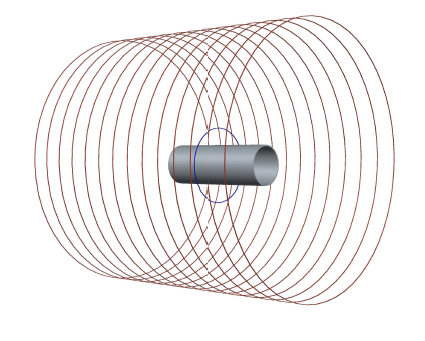
\includegraphics[width=0.8\textwidth]{geometry.PNG}
    \caption{Axial shielding factor measurement setup. The witness
      cylinder with a radius of 2.54~cm and a length of 15.2~cm is placed
      inside a solenoid with a radius and a half length of
      17.44~cm. The axis of symmetry is along the $z$-axis. The
      windings of the solenoid is shown in red. The blue coil with one
      turn is coupled to the witness cylinder and it has a radius of
      5~cm.  }
% Note to Jeff (self): fix this figure caption!!!
% (Need to look at it in the pdf form to think more about it.)
    \label{fig:geometry}
    \end{center}
\end{figure}

As shall be described in Section~\ref{sec:axialsyst}, a concern in the
measurement was changes in the field measured by the fluxgate that
could arise due from motion of the system components, or other
temperature dependences.  This could generate a false slope with
temperature that might incorrectly be interpreted as a change in the
magnetic properties of the witness cylinder.

To address possible motion of the witness cylinder with respect to the
field generation system, another coil was wound on a plastic holder
mounted rigidly to the witness cylinder.  The coil was one loop of
copper wire with a radius of 5~cm. The loop coil holder had inner
radius of 2.7~cm and an outer radius of about 5~cm.  Plastic set
screws in the holder fixed the loop coil to be coaxial with the
witness cylinder.

Systematic differences in the results from the two coils (the
solenoidal coil, and the loop coil) were used to search for motion
artifacts.  As well, some differences could arise due to the different
magnetic field produced by each coil, and so such measurements could
reveal a dependence on the profile of the applied magnetic field.  In
the end, no conclusive difference in the results from either coil
could be found.  This is described further in
Section~\ref{sec:axialsyst}.


\subsubsection{Temperature measurement and data acquisition}


%%%%%%%%%%%%%%%%%%%%%%%%%%%%%%%%%%%%%%%%%%%%%%%%%%%%%%%%%%
% It has been moved up from the systematic error section
%%%%%%%%%%%%%%%%%%%%%%%%%%%%%%%%%%%%%%%%%%%%%%%%%%%%%%%%%%
%
%The mu-metal alloy has a thermal conductivity of 0.35
%W/(cm$\cdot$K). Therefore, four thermocouples placed on different
%spots on the witness cylinder to correct for small temperature
%differences on each end of the witness cylinder.  In these
%measurements, the farther side of the passive shields had the end caps
%while the other side was left open to give access to the interior
%region. Based on the magnetic field maps inside the passive shields,
%for 10 $\mu$T applied magnetic field, the stability of the field was
%to 0.1 $\mu$T level and the magnetic field was even more stable closer
%to the closed side of the passive shields. Therefore the witness
%cylinder was pushed to the side with the end caps on the passive
%shields.


The temperature of the witness cylinder was measured by attaching four
thermocouples at different points along the outside of the cylinder.
To reduce any potential magnetic contamination, T-type thermocouples
were used, which have copper and constantan conductors.  (K-type
thermocouples are magnetic.)  Two thermocouples were attached to the
edges of the witness cylinder and the other two were attached on
opposite sides in the middle.  This allowed us to observe the
temperature gradient along the witness cylinder.

Thermocouple readings were recorded by a National Instruments NI-9211
temperature input module.  The magnetic field (signified by the
lock-in amplifier readout) and the temperature were recorded at a rate
of 0.2~Hz.

Temperature variations in the experiment were driven by ambient
temperature changes in the room, although forced air and other
techiques were also tested.  These are described further in
Section~\ref{sec:axialsyst}.


\subsubsection{Data and Interpretation}

An example of the typical data acquired is shown in
Fig.~\ref{fig:B_vs_Temp}.  The field amplitude produced by the
solenoid was 2.6~$\mu$T, at a frequency of 1~Hz.
Fig.~\ref{fig:B_vs_Temp}(a) shows the temperature of the witness
cylinder over a four-day measurement.  The temperature changes are
about 3.5~K and are caused by temperature variations of the
laboratory.
% The following statement belongs more in the systematic errors section:
%
% For $f\lesssim 1$~Hz most of the measured fluxgate signal is in the
% in-phase component.
%
The magnetic field $B$ is anti-correlated with the temperature trend
in an shown in Fig.~\ref{fig:B_vs_Temp}(b).  Here, $B$ is the sum, in
quadrature, of the amplitudes of the in-phase and out-of-phase
components.  Magnetic field is then interpreted to depend on the
temperature, and they are graphed as a function of one another in
Fig.~\ref{fig:B_vs_Temp}(c).  The slope of Fig.~\ref{fig:B_vs_Temp}(c)
has been calculated using a linear fit to the data.  In this
measurement, the slope is found to be
$\frac{1}{|B|}\frac{d|B|}{dT}\simeq -1.5\%$/K.

Deviations from the linear straight-line dependence can be seen in the
data.  For example at the start of the data-taking, the slope is
almost zero.  This is typical of the data that we acquired, that the
magnetic field as a function of temperature would not necessarily lie
along a straight line, but rather would have different slope
temporarily after changing the sign of the temperature slope with
time.

Another feature of the data was that, on subsequent similar
measurements, the value of the slope would not be the same, on a
measurement-to-measurement basis.

A comprehensive set of systematic studies of the factors affecting the
slope were performed, and these are presented in
Section~\ref{sec:axialsyst}.  A basic summary of those studies was
that no external parameter was found that could explain the periodic
changes in slope that were observed.  Based on these studies, we
expect the change in slope is either due to an irreproducibility in
the magnetic properties of the material, or due to an uncharacterized
systematic error such as a long-time mechanical relaxation of some
element of the apparatus.

To express this inherent uncertainty in the slope, we phrase our
result as a range of slopes that were typical of data acquired over
time periods of $\sim$ days.  In general, we measured
0.3\%/K~$<\vert\frac{1}{B}\frac{dB}{dT}\vert<$~2.3\%/K with the sign
% Jeff got to here on pass 2.
% question for Taraneh: should be solenoidal coil only? or what's the
% answer for solenoidal coils as compared to loop coil?  answer from
% Jeff and Taraneh, so far: this needs to be fixed.  We should put
% both measurements up here and explain the difference.
being negative.  The range also encompasses the typical deviation from
a linear $B(T)$ in the data (for example, those seen in
Fig.~\ref{fig:B_vs_Temp}(c).).  Since the data cannot be embodied by a
single temperature slope, the experiment tends to set a scale and sign
for the possible temperature dependence, rather than a value.

\begin{figure}
\begin{center}
   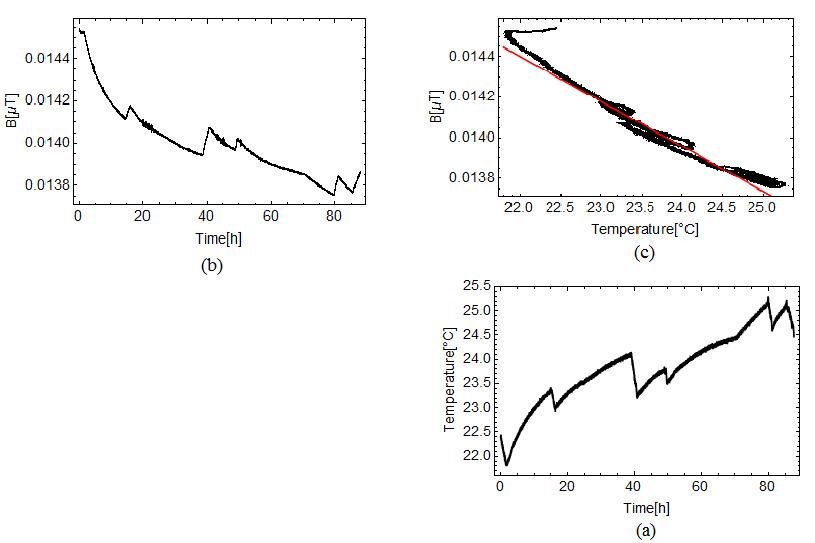
\includegraphics[width=0.5\textwidth]{B_vs_T.png}
% Taraneh to do: vertical label should likely be ``B amplitude'' or
% ``amplitude of measured field'', to make it clear that this has been
% multiplied by sqrt(2).  Either that, or the sqrt(2) should be
% removed to avoid inconsistency with the transformer measurements
% presented later.
    \caption{Ambient temperature and shielded magnetic field
      amplitude, measured over a 90 hour period. (a) temperature of
      the witness cylinder as a function of time.  (b) magnetic field
      amplitude measured by fluxgate at center of witness cylinder
      versus time.  (c) magnetic field versus temperature. The red
      line in (c) is a linear fit to data. At 22$^\circ$C,
      $\frac{1}{|B|}\frac{d|B|}{dT}=-1.5\%$/K.}
% This was actually measured by the local coil!!!
% This was actually measured by the local coil!!!
    \label{fig:B_vs_Temp}
    \end{center}
\end{figure} 

% This was actually measured by the local coil!!!
% This was actually measured by the local coil!!!

% Taraneh says: Several data from March 2015 is now added to the long
% report on Plone. We might need to consider replacing this graph with
% another one. I am aware of the fact that the graphs in the long
% report are not publication quality. But once we decide on some
% particular data, I will make nicer looking graphs.

\subsubsection{Systematic Studies\label{sec:axialsyst}}

\paragraph{Methods of Temperature Variation}

In addition to ambient temperature changes, we tried other methods of
forced temperature change.  In one design, Tygon tubing was wrapped
around the witness cylinder in a spiral pattern to flow water whose
temperature could be controlled.  Mechanical stability issues clearly
dominated the systematic uncertainty in that measurement.  When water
was flowing, the flexibility of the tubing caused a movement in the
witness cylinder.  The motion was itself temperature-dependent because
warmer water caused the tubing to become more supple.  To address this
effect, the tubes were replaced by copper tubing.  But in this case,
the challenge was to create enough contact between the tubes and the
witness cylinder which was not successful. In another design, a TEC
was replaced with the tubing. The main issue with this design was that
it did not provide enough cooling for the witness cylinder and also it
was creating only local temperature changes on the witness
cylinder. In addition, despite of using heat sinks, the heat created
by the TEC itself made it very inefficient.  We also tried using
forced air to heat the witness cylinder.  This worked rather well, but
the heating had to be done slowly in order to avoid temperature
gradients across the apparatus, including the witness cylinder.  In
the end, using the ambient temperature changes in the room gave the
most reproducible results.  These followed a relatively stable diurnal
cycle with the function of the building's air conditioning system.

Although for most of the measurements the general trend of $B(T)$
graphs was consistent, the shape and positions of the nonlinear parts
of $B-T$ graphs were changing.  The changes in the $B$ vs.~temperature
slope always correlate with sharper changes in the temperature with
time.  The effect is most pronounced when a temperature that is
decreasing with time suddenly changes to increasing, or vice-versa.
However, we have incorporated the uncertainty from this effect into
our stated range of values.




%\paragraph{Final Design} 

% This has all been said and could be deleted, I think:

%final design
%The final design included the witness cylinder, which was placed with
%a holder inside the innermost prototype passive shield. The
%temperature variations of the witness cylinder was due to the
%temperature changes in the room which was following the on and off
%cycles of the building air conditioner.
%A Bartington magnetic field
%sensor (fluxgate) was hold inside the witness cylinder at the centre
%by plastic holder. The signal from the sensor was then demodulated by
%an SRS830 lock-in amplifier. To convert the final measured voltage
%from the sensor to $\mu$T, the sum in quadratures of the in-phase and
%out of phase components of the lock-in amplifier was multiplied by the
%scaling factor on the magnetic field sensor which is 7 $\mu$T/V.


%%%%%%%%%%%%%%%%%%%%%%%%%%%%%%%%%%%%%%%%%%%%%%%%%%%%%%%%%%%%%%%%%%%%%%
% This is all new and needs to move up to the apparatus section: (done)
%%%%%%%%%%%%%%%%%%%%%%%%%%%%%%%%%%%%%%%%%%%%%%%%%%%%%%%%%%%%%%%%%%%%%%
% The
% mu-metal alloy has a thermal conductivity of 0.35
% W/(cm$\cdot$K). Therefore, four thermocouples placed on different
% spots on the witness cylinder to correct for small temperature
% differences on each end of the witness cylinder.  In these
% measurements, the farther side of the passive shields had the end caps
% while the other side was left open to give access to the interior
% region. Based on the magnetic field maps inside the passive shields,
% for 10 $\mu$T applied magnetic field, the stability of the field was
% to 0.1 $\mu$T level and the magnetic field was even more stable closer
% to the closed side of the passive shields. Therefore the witness
% cylinder was pushed to the side with the end caps on the passive
% shields.
%%%%%%%%%%%%%%%%%%%%%%%%%%%%%%%%%%%%%%%%%%%%%%%%%%%%%%%%%%%%%%%%%%%%%%

% Another list
% - amplitude measurement on oscilloscope (no lock-in). (done)
% - speed of temperature change? temperature homogeneity?  (not here yet) 
% - other methods of cooling and why they didn't work. (not here yet)(done)
% - magnetic contamination by thermocouples (done)

% The above list maybe explains other possible variations on the
% method that you tried that all seemed to have worse systematic
% errors.

% Then, a list of systematic errors once you settled on the final
% measurement technique...

% - field profile/homogeneity (done)
% - mechanical stability (done)
% - thermal expansion (done)
% - temperature dependence of fluxgate and SCU (done)
% - temperature dependence of lock-in (done)
% - temperature dependence of coil resistance (not here yet) (done)
%    - Cupron/etc. study. plus
%    - measuring across the precision resistor
% - null measurement (Cu, and why it doesn't give the whole story, not here yet) (done)
% - effect of endcaps? (influence of external fields, not here yet)(done)
% - temperature dependence of reaction factor (negligible, not here yet)(done)
% - degaussing (not here yet)(done)
% - measurements on different witness cylinders? (not here yet)(done)
% - vibrations of the building?(done)
% - ...
%
% Another list is on the oldelog somewhere.  Please find it.
% The above list is longer and inclusive of the old list.
% See oldelog entry 141 in Magnetic Fields.
%
% This list of systematics is addressed now...

\paragraph{Field profile dependence and mechanical stability}

As mentioned earlier, a concern in the measurement was that motion of
the witness cylinder, the solenoidal coil, and the innermost magnetic
shield relative to one another could generate a false temperature
slope.  Another concern was that the spatial variation of the magnetic
field generated by the coil could somehow affect the measurement.  To
address these concerns, a loop coil rigidly mounted to the witness
cylinder was used to search for any differences compared to results
measured with the solenoidal coil.

The result of this study was that it did not reduce the typical slopes
measured, nor improve their reproducibility.  In the end, repeated
measurements of temperature slopes using the loop coil fell in the
range
0.4\%/K~$<\vert\frac{1}{B}\frac{dB}{dT}\vert<$~1.5\%/K.
% 0.5 is from Page 15 of Taraneh's summary.
% 0.4 is seen on Page 34 of Taraneh's logbook, Volume 1, Aug 2014-Dec 2015.
% 1.5 is from the Figure showed in the paper (page 14 of Taraneh's summary).
Similar measurements for the solenoidal coil yielded
0.3\%/K~$<\vert\frac{1}{B}\frac{dB}{dT}\vert<$~0.8\%/K.
% 0.3 is from Page 30 of Taraneh's summary
% 0.75 is from Page 34 of Taraneh's logbook, Volume 1, Aug 2014-Dec 2015.

% Jeff notes: these results should be stated as the primary results,
% right after/near the figure of the data.

% Taraneh to do: make a comment on H, right here, right now.  We
% should have a value for both the solenoidal coil and the loop coil.
% You might have to force Jeff to get it from his FEMM simulations.

In general, the slopes measured with the loop coil are larger than for
the solenoidal coil.  A partial explanation of this difference is
offered by the field profile generated by each coil, and its
interaction with the witness cylinder.  This is addressed further in
Section~\ref{sec:axialsims}.

However, the range of slopes measured in different trials still varied
within the stated ranges.  We conclude that whatever is causing the
slopes to change periodically is likely unrelated to motion of the
witness cylinder relative to the magnetic elements in the system.


% What is the value of the systematic error deduced from this study?
% I would say that the result of this study was that we got similar
% data to Fig. 3(c).  Therefore the systematic error due to field
% profile is smaller than the unknown systematic error of Fig. 3(c)
% and similar figures.  also partly addresses possible changes in
% reaction factor with temperature. (done)

Other potential motion artifacts due to thermal expansion of
components was also considered.  The thermal expansion coefficient of
mu-metal is $\sim$10~ppm/K~\cite{kruppvdm}.  However if the witness
cylinder expands uniformly in both thickness and radius, the shielding
factor is to first order unchanged.  In general, even unnatural
asymmetric and twisting motions of the fluxgate sensor and witness
cylinder tended to generate temperature slopes in the magnetic field
at the level $<30$~ppm/K.  The general homogeneity of the magnetic
field at the fluxgate sensor position and of the applied magnetic
field within which the witness cylinder was placed aided in minimizing
motion artifacts.

% http://nuclear.uwinnipeg.ca/oldelog/Magnetic+Fields/141
%As another mechanical stability study, the movement of the Bartington
%fluxgate flying lead due to thermal expansion was estimated. If the
%fluxgate flying lead move about 1 mm normal to its axis of symmetry
%which is parallel to the axis of the witness cylinder, the magnetic
%field will change about 30~ppm/K over 20~K temperature changes.

% %vibration
% Since the experiment site is located at the heart of downtown it is
% also possible that vibrations of the building affected the experiment
%setup and its machanical stability.
% Jeff says:  I can't think of much to say here.


%effect of the end caps

% Taraneh's version:

% In this experiment, one side of our prototype passive shield was
% closed with the end caps while the other side left open for easier
% access to the interior region. The result of the magnetic field map
% inside the prototype shield when the solenoid was turned on showed
% that closer to the far side of the shield, where the shield is closed,
% the magnetic field is more uniform. For a 10$\mu$T applied magnetic
% field the maximum change of the magnetic field along the axis of the
% passive shield was the order of 0.1~$\mu$T.  Therefore the witness
% cylinder was pushed to the far side of the prototype shield to reduce
% the non uniformity of the magnetic field.
% This is from oldElog entry 146: field map by Andrew Harrison

% Jeff's version (slightly shorter)

% As stated in Section~\ref{sec:axialapparatus}, the measurements were
% conducted within the magnetically shielded volume inside our
% prototype magnetic shields.  Most of the measurements were conducted
% with the endcaps of this shielding system removed on one side.  No
% systematic effect was found to arise from the removal of the
% endcaps.  The only effect was that the field produced by the
% solenoid was somewhat less homogeneous, which could easily be
% accounted for by moving the witness cylinder slightly closer to the
% side which has its endcaps on.  This was verified by measuring a
% magnetic field map of the region.

% Jeff's final version

% say nothing - this is an unimportant detail.  It had no effect on
% the measurement.  As far as we know, we would get the same value
% endcaps on or off.  I think it is more confusing to raise some
% possible issue about it and then say it wasn't a problem.

%temperature dependence of reaction factor
As the witness cylinder was put through its diurnal heating and
cooling cycles, so too was the magnetic shield within which the
apparatus was placed.  Since this magnetic shield is used as a flux
return, especially for the solenoidal coil, a concern could be that
the measurement confounds temperature dependence of the flux return
with the temperature dependence of the shielding factor of the
solenoid.  We want to clarify that this cannot be the case: any change
in $\mu$ of the flux return will have an exceedingly small effect on
the field produced by the solenoid.  This is perhaps best demonstrated
by Fig. \ref{fig:Magnetic_Field}, where the reaction factor in a
similar cylindrical geometry is graphed as a function of $\mu$.  Based
on our measurements, this limits systematic errors from such an effect
to be $<200$~ppm/K.

% This number above comes from:

% mu/B dB/dmu = 0.01

% times

% 1/mu dmu/dT < 2%/K

%degaussing
The magnetization of the witness cylinder changes the magnetic
permeability of the material and so the shielding factor changes.  Our
studies of degaussing the witness cylinder were consistent with
studies that we will report in
Section~\ref{sec:transformerdegaussing}.  Essentially, if the shields
were degaussed, or if they were left for long periods of time in the
small AC field generated by the solenoid, the results for temperature
dependences were similar.  Improper degaussing procedures were found
to induce long-term drifts in the measurement, uncorrelated with
temperature.  We do not include such data when quoting our
measurements of temperature slopes.  We do think that part of the
range of slopes that we measured is due to the magnetic properties of
the material, and that it is possible that some of this range is yet
due to insufficient degaussing on our part.  This is something we plan
to improve in planned future experiments on DC field stability.



\paragraph{Temperature slopes of various components of the apparatus}

The temperature coefficients of various components that could affect
the measurement were also considered.

The Mag-03IEL70 Bartington magnetic field sensor has a scaling
temperature coefficient of 15~ppm/K~\cite{bib:bartman}.  There is also
temperature coefficient for the offset of these sensors, but this is
irrelevant for this measurement because of the AC fields and
demodulation technique used.

The SRS830 lock-in amplifier has 50~ppm/K amplitude
stability~\cite{bib:lockin}.
% We did this for the transformer technique.
% Yes, but I think it is valid for this measurement as well, so let's put
% it here.
To further test this, the lock-in amplifier was connected to the coil
through a 1~$\Omega$ resistor with small temperature coefficient.  The
voltage across the resistor was measured with the lock-in amplifier
itself.  Any change would then be interpreted as a change in the
current supplied to the coil by the lock-in amplifier.  The measured
temperature dependence was always $<0.1$\%/K.

% To address this effect, another measurement conducted with local coil
% with Cupron wire windings. Cupron has higher resistivity compared to
% copper wires. The results showed no linear correlation between the
% measured magnetic field and the temperature of the witness cylinder.

% Taraneh asks:  The results?  Stride gum?  What to say?

% Jeff responds: I am not sure what to say about these results.  We
% didn't do the same measurement with the 1 Ohm resistor, I think, so
% it's hard to say if it was a problem with the temperature
% coefficient of resistance, or some geometrical change due to
% temperature change, or what.  Basically it is a confusing result in
% a somewhat weird experimental setup.

%Taraneh: I calculated from the long summary
The stability of the system was also tested by replacing the mu-metal
witness cylinder with a copper cylinder of very similar dimensions.
All other components of the system were the same.  The apparatus was
then run through its usual experimental cycle over several days.  For
all such measurements the temperature dependence of the demodulated
magnetic was $<0.1$\%/K.  This kind of measurement is unable to
address all possible systematic uncertainties.  For example, if moving
the mu-metal witness cylinder due to some thermal expansion would
change the field at the site of the fluxgate, moving the copper
cylinder will not make the same change.  Nonetheless it is an
encouraging result that the system does not measure a strong
temperature dependence of the magnetic field when no mu-metal witness
cylinder is present.  The magnitude of the magnetic field measured at
the fluxgate sensor was larger during these measurements because of
the lack of magnetic shielding from the copper.  So, in some tests the
magnetic field generated by the reference channel of the lock-in
amplifier was reduced to search for any problems arising from smaller
fluxgate signals.  No difference was seen within the upper bound
stated above.

\paragraph{Different Witness Cylinders}

The manufacturer of our prototype magnetic shields provided us with
three witness cylinders.  All three were used in these measurements.
Different cylinders possessed systematically different temperature
slopes, although always within the ranges quoted above.  These changes
are believed to arise from the manufacturing and annealing process.
It is known that the take-out temperature in the annealing process has
a strong effect on the temperature slopes measured at
50~Hz~\cite{bib:kruppdatasheet}.



% Two possibilities:

% 1. unknown systematic error(s)

% 2. complicated material properties that don't follow a straight line
% could depend on material history themselves.

% Therefore we state a range which should be indicative of the scale
% of possible temperature dependence.


\subsubsection{Geometry correction and determination of $\mu(T)$\label{sec:axialsims}}

To relate the data to $\mu(T)$, the shielding factor of the witness
cylinder as a function of $\mu$ must be known.  Finite element
simulations in FEMM and OPERA were performed to determine this factor.

Combining the measurement and the simulations, the temperature
dependence of the effective $\mu$ (at $\mu=20 000$, which is consistent
with our measurements) can be calculated by
\begin{equation}
\frac{1}{\mu}\frac{d\mu}{dT}=-\frac{\frac{1}{B}\frac{dB}{dT}}{\frac{\mu}{B}\frac{dB}{d\mu}}.
\end{equation}

From the simulations the ratio $\frac{\mu}{B} \frac{dB}{d\mu}$ was
calculated.  A linear model of the material was used where
$\bold{B}=\mu \bold{H}$ and $\mu$ is a constant independent of
$\bold{H}$.  The term $\frac{\mu}{B}\frac{dB}{d\mu}\neq 1$ because the
witness cylinders are open ended, and hence even for very large
$\mu\rightarrow\infty$ the shielding factor asymptotically approaches
a constant rather than infinity.

The simulations differed slightly in their results, dependent on
whether OPERA or FEMM was used, and whether the solenoidal coil or
loop coil were used.

Based on the simulations, the result is
$\frac{\mu}{B}\frac{dB}{d\mu}=0.42-0.50$ for the solenoidal coil, with
the lower value being given by FEMM and the upper value being given by
a 3D OPERA simulation, for identical geometries.  This is somewhat
lower than the value suggested by
Paperno~\cite{bib:paperno-open-ended} in his fits to simulations
performed in OPERA, which we estimate to be 0.6.  We adopt our value
since it is difficult to determine precisely from
Ref.~\cite{bib:paperno-open-ended}.  For the loop coil, we determine
$\frac{\mu}{B}\frac{dB}{d\mu}=0.56-0.65$, the range being given again
by a difference between FEMM and OPERA. These are presented in the second left column of Table~\ref{tab:axialsummary}. The third column from left summarizes the values of $B(T)$ measurements for both coil geometries discussed earlier in this section. The last column is the ratio of the third to the second column. 



\begin{table}
\begin{tabular}{|c|c|c|c|}
\hline 
  & $\vert \frac{\mu}{B}\frac{dB}{d\mu}\vert$ & $\vert \frac{1}{B} \frac{dB}{dT}\vert$~(\%/K) & $\frac{1}{\mu}\frac{d\mu}{dT}$~(\%/K) \\ 
\hline 
Solenoidal Coil & 0.42-0.50 & 0.3-0.8 & 0.6-1.9 \\ 
\hline 
Loop Coil & 0.56-0.65 & 0.4-1.5 & 0.6-2.7 \\ 
\hline 
\end{tabular} 
%\caption{A table to be filled in by Taraneh, and described in this
% caption and the surrounding text.}
\caption{The result of OPERA and FEMM simulations and the shielding factor measurement as well as the temperature dependence of $\mu$ for solenoidal and loop coil is summarized here. More detail is provided in the text.}
\label{tab:axialsummary}

\end{table}


Taking all these systematics into account, in this method it was found
that 0.6\%/K~$\lesssim\frac{1}{\mu}\frac{d\mu}{dT}\lesssim 2.7\%$/K.
This is quoted for a typical $H$ amplitude of XXX and a frequency of
1~Hz.

% Taraneh to do: look up number XXX for $H$.



%\begin{itemize}
%\item Describe experimental setup and important considerations
%  (e.g. relationship of data to effective $\mu$)
%\item Explain B, H, f, and dominant systematic effects.
%\item One figure of experimental setup?
%\item One data graph?
%\item State overall result and systematic error.
%\end{itemize}


% Transformer core measurements Section moved to transformer.tex


\subsection{Transformer Core Measurements}
\label{sec:transformer}

As an alternative method of measuring changes in $\mu$, a method
similar to the standard method of magnetic materials characterization
via magnetic induction was used.  In this measurement technique, the
witness cylinder was used as the core of a transformer.  Two coils
(primary and secondary) were wound on the witness cylinder using
multistranded 20-gauge copper wire.  The windings were made as tight
as possible, but not so tight as to potentially stress the material.
The windings were not potted in place.

Three witness cylinders were tested.  Data were acquired
using different numbers of turns on both the primary and secondary
coils (from 6 to 48 on the primary, and from 7 to 24 on the
secondary).
% Table 9 on page 65 of Taraneh's report shows the different windings.
% Can guess which core is which.

%In the end, a transformer with 48 windings on the primary and 21
%windings on the secondary was used.

%This enabled more saturation of the material.

The primary coil generated an AC magnetic field as a function of time
$H(t)$, while the secondary coil was used to measure the emf induced
by the time-varying magnetic flux proportional to $dB(t)/dt$.  To a
good approximation
\begin{equation}
H_m(t)=\frac{N_pI(t)}{2\pi R}
\end{equation}
where $N_p$ is the number of turns in the primary, $I(t)$ is the
current in the primary, and $R$ is the radius of the witness cylinder,
and
\begin{equation}
\frac{dB_m(t)}{dt}=\dot{B}_m(t)=\frac{V(t)}{t\ell}
\label{eqn:bdot}
\end{equation}
where $V(t)$ is the voltage generated in the secondary, and $t$ and
$\ell$ are the thickness and length of the witness cylinder.  For a
sinusoidal drive current $I(t)$, and under the assumption that
$B_m(t)=\mu H_m(t)$ with $\mu$ being a constant, the voltage generated
in the secondary $V(t)$ should be sinusoidal and out of phase with the
primary current.

The internal oscillator of an SR830 lock-in amplifier was used to
generate $I(t)$.  This was monitored by measuring the voltage across a
1~$\Omega$ resistor with small temperature coefficient in the primary
loop.  The lock-in amplifier was then used to demodulate $V(t)$ into
its in-phase $V_X$ and out-of-phase $V_Y$ components (or equivalently
$\dot{B}_m(t)$ being demodulated into $\dot{B}_{m,X}$ and
$\dot{B}_{m,Y}$, as in equation~(\ref{eqn:bdot})).  The experiment was
done at 1~Hz with $H_m(t)$ as small as possible, typically 0.1~A/m in
amplitude, to measure the slope of the minor $B_m-H_m$ loops near the
origin of the $B_m-H_m$ space.

The temperature of the core was measured continuously using the same
thermocouple arrangement described previously.  Measurements of $V_Y$
as a function of temperature would then signify a change in $\mu$ with
temperature.  In general, we used ambient temperature variations for
the measurements, similar to the procedure used for our axial
shielding factor measurements.

% Although we would have preferred to measure at even lower frequencies
% and amplitudes, these settings were found to be the minimum possible
% before noise would make it impossible to measurement the long-term
% (hours) evolution of the $X$ and $Y$ readings.

The naive expectation is that the out-of-phase $V_Y$ component should
signify a non-zero $\mu$, and the in-phase $V_X$ component should be
zero.  In practice, due to a combination of saturation, hysteresis,
eddy-current losses, and skin-depth effects, the $V_X$ component is
nonzero.  It was found experimentally that keeping the amplitude of
$H_m(t)$ small compared to the apparent coercivity ($\sim 3$~A/m for
the 0.16~cm thick material at 1~Hz frequencies) ensured that the $V_Y$
component was larger than the $V_X$ component.  This is displayed
graphically in Fig.~\ref{fig:data_and_simulation}, where the
dependence of $\dot{B}_{m,Y}$ and $\dot{B}_{m,X}$ on the amplitude of
the applied $H_m(t)$ is displayed, for a driving frequency of 1~Hz.
Clearly the value of $\dot{B}_{m,X}$ can be considerable compared to
$\dot{B}_{m,Y}$, for larger $H_m$ amplitudes near the coercivity.  At
larger amplitudes, the material goes into saturation.  Both
$\dot{B}_{m,Y}$ and $\dot{B}_{m,X}$ eventually decrease as expected at
amplitudes much greater than the coercivity.

To understand the behavior in Fig.~\ref{fig:data_and_simulation}, a
theoretical model of the hysteresis based on the work of
Jiles~\cite{bib:jiles} was used.  The model contains a number of
adjustable parameters.  We adjusted the parameters based on our
measurements of $B_m-H_m$ loops including the initial magnetization
curve.  These measurements were performed separately from our lock-in
amplifier measurements, using an arbitrary function generator and a
digital oscilloscope to acquire them.  The measurements were done at
frequencies from 0.01 to 10~Hz.  It was found that the frequency
dependence predicted by Ref.~\cite{bib:jiles} gave relatively good
agreement with the measured $B_m-H_m$ loops once the five original
(Jiles-Atherton~\cite{bib:jiles-atherton}) parameters were tuned.

For the parameters of the (static) Jiles-Atherton model, we used
$B_s=0.45$~T, $a=3.75$~A/m, $k=2.4$~A/m, $\alpha=2\times 10^{-6}$,
$c=0.05$, which were tuned to our $B_m-H_m$ curve measurements.  For
classical losses, we used the parameters $\rho=5.7\times
10^{-7}~\Omega\cdot$m, $d=1.6$~mm (the thickness of the material), and
$\beta=6$ (geometry factor).  These parameters were not tuned, but
taken from data.  For anomalous losses we used the parameters
$w=0.005$~m and $H_0=0.0075$~A/m, which we also did not tune, instead
relying on the tuning performed in Ref.~\cite{bib:jiles}.

These parameters were then used to model the measurement presented in
Fig.~\ref{fig:data_and_simulation}, including the lock-in amplifier
function.  As shown in Fig.~\ref{fig:data_and_simulation}, trends in
the measurements and simulations are fairly consistent.  The sign of
$\dot{B}_{m,X}$ relative to $\dot{B}_{m,Y}$ is also correctly
predicted by the model (we have adjusted them both to be positive, for
graphing purposes).  We expect that with further tuning of the model,
even better agreement could be achieved.

\begin{figure}[h!]
  \begin{center}
    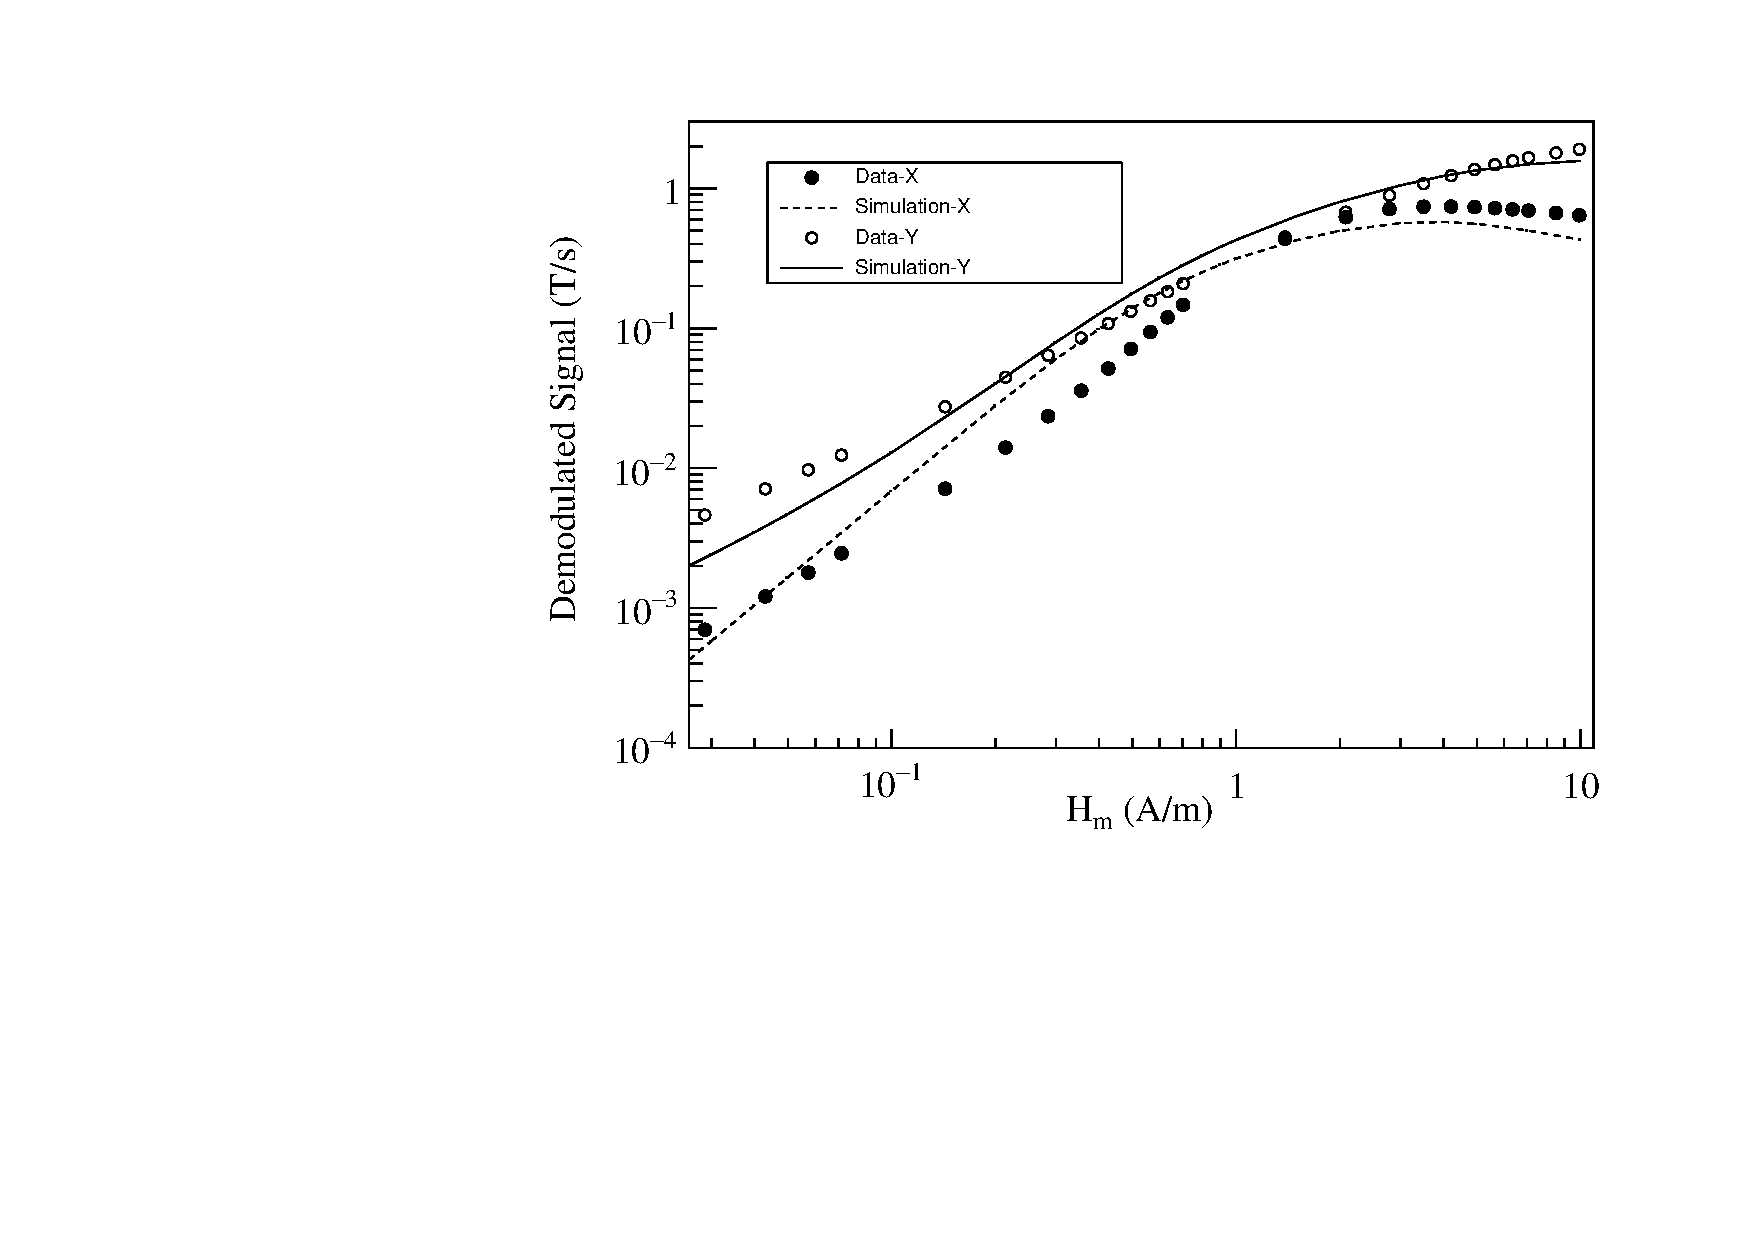
\includegraphics[width=\textwidth]{Jiles_and_data.pdf}
    \caption{$\dot{B}_{m,X}$ and $\dot{B}_{m,Y}$ as a function of
      amplitude of the applied $H_m$ field at 1~Hz.  Points show the
      acquired data.  Curves display the simulation based on the model
      described in the text.}
    \label{fig:data_and_simulation}
  \end{center}
\end{figure} 

Jiles' model makes no prediction of the temperature dependence of the
parameters.  Ideally, the temperature dependence of $\dot{B}_{m,Y}$
and $\dot{B}_{m,X}$ under various conditions could be used to map out
the temperature dependence of the parameters.  However, this is beyond
the scope of the present work.

We make the simplifying assumption that temperature dependence of
$\dot{B}_{m,Y}$ may be approximately interpreted as the temperature
dependence of a single parameter $\mu$, i.e. that
\begin{equation}
\frac{1}{\dot{B}_{m,Y}}\frac{d\dot{B}_{m,Y}}{dT}=\frac{1}{\mu}\frac{d\mu}{dT}.
\end{equation}
This is justified in part by our selection of measurement parameters
(the amplitude of $H_m=0.1$~A/m and a measurement frequency of 1~Hz)
which ensure that $\dot{B}_{m,Y}$ dominates over $\dot{B}_{m,X}$.

We assign no additional systematic error for this simplification, and
all our results are subject to this caveat.  We comment further that
in our measurements of the axial shielding factor (presented in
Section~\ref{sec:axial}), the same caveat exists.  In that case the
in-phase component dominates the demodulated fluxgate signal.  In a
sense, measuring $\mu(T)$ itself is always an approximation, because
it is actually the parameters of minor loops in a hysteresis curve
which are measured.  In reality, our results may be interpreted as a
measure of the temperature-dependence of the slopes of minor loops
driven by the stated $H_m$.

Measurements of $\frac{1}{\dot{B}_{m,Y}}\frac{d\dot{B}_{m,Y}}{dT}$ as
a function of $T$ were made.  In general, the data mimicked the
behavior of the axial shielding factor measurements, giving a similar
level of linearity with temperature as the data displayed in
Fig.~\ref{fig:B_vs_Temp}.  Other similar behaviors to those
measurements were also observed, for example: (a) when the temperature
slope changed sign, $\dot{B}_{m,Y}$ would temporarily give a different
slope with temperature, (b) the measured value of
$\frac{1}{\dot{B}_{m,Y}}\frac{d\dot{B}_{m,Y}}{dT}$ depended on a
variety of factors, most notably a dependence on which of the three
witness cylinders was used for the measurement, and on differences
between subsequent measurements using the same cylinder.

Based on a number of measurements with different cores and windings,
the data showed a range of $0.1-2.1$\%/K for
$\frac{1}{\mu}\frac{d\mu}{dT}=\frac{1}{\dot{B}_{m,Y}}\frac{d\dot{B}_{m,Y}}{dT}$,
again naively assuming the material to be linear as discussed above.
The sign of the slope of $\mu(T)$ was the same as the axial shielding
factor technique.

A dominant source of variation between results in this method arose
from properties inherent to each witness cylinder.  One of the
cylinders gave temperature slopes consistently larger
$\frac{1}{\mu}\frac{d\mu}{dT}\sim 1.2-2.1$\%/K than the other two
$\frac{1}{\mu}\frac{d\mu}{dT}\sim 0.1-0.7$\%/K.  We expect this
indicates some difference in the annealing process or subsequent
treatment of this cylinder, although to our knowledge the treatment
was controlled the same as for the other two cylinders.  Since our
goal is to provide input to future EDM experiments on the likely scale
of the temperature dependence of $\mu$ that they can expect, we phrase
our result as a range covering all these results.

Detailed measurements of the effect of degaussing were conducted for
this geometry.  The ability to degauss led us ultimately to select a
larger number of primary turns (48) so that we could fully saturate
the core using only the lock-in amplifier reference output as a
current source.  A computer program was used to control the lock-in
amplifier in order to implement degaussing.  A sine wave with the
measurement frequency (typically 1~Hz) was applied at the maximum
lock-in output power.  Over the course of several thousand
oscillations, the amplitude was decreased linearly to the measurement
amplitude ($\sim 0.1$~A/m).  After degaussing with parameters
consistent with the recommendations of
Refs.~\cite{bib:thiel,bib:altarev2015}, the measured temperature
slopes were consistent with our previous measurements where no
degaussing was done.

Other systematic errors found to contribute at the $<0.1\%$/K level
were: motion of the primary and secondary windings, stability of the
lock-in amplifier and its current source, and stability of background
noise sources.

To summarize, the dominant systematic effects arose due to different
similarly prepared cores giving different results, and due to
variations in the measured slopes in multiple measurements on the same
core.  The second of these is essentially the same error encountered
in our axial shielding factor measurements.  We expect it has the same
source; it is possibly a property of the material, or an additional
unknown systematic uncertainty.


\subsection{Summary of $\mu(T)$}
%Insert Summary Here.
The overall error bar in $\mu$ from both measurement techniques is 0.1\%/K $\leq \frac{1}{\mu}\frac{d\mu}{dT} \leq$ 2.3 \%/K and it is consistent with previous data.
Comparing to the static nEDM experiment with $f < 0.01$ Hz, these measurements are mostly done at frequencies close to 1 Hz. Hence, the effective $\mu$ extracted from these type of experiments give
only a qualitative information on the actual nEDM experiment situation and to reach higher accuracy the nEDM experiment has to be built. 
\section{Summary and Conclusions}
The magnetic field internal to the passive shields as a function of $\mu$ for spherical geometry with parameters close to the ILL nEDM experiment has been analytically calculated and compared to axis-symmetric simulations with similar parameters for both spherical and cylindrical geometries. For spherical geometry $\frac{dB_0}{d\mu}\sim 4 \times 10^{-13}$ and it can be much reduced for the shield coupled coils.
The temperature dependence of $\mu$ has been measured by two different techniques using open-ended mu-metal cylinders with 6 inches in length. The overall result gives 0.1\%/K$\frac{1}{\mu}\frac{d\mu}{dT}$2.3 \%/K. Because of the different values in $f$, $B$ and $H$ fields as opposed to the nEDM experiments, these  measurements help to set the specifications for the actual nEDM setup. The nonlinearities in the witness cylinder material such as hysteresis dominated the systematic uncertainties at both measurements and so it was difficult to achieve consistent sub-percent determinations although the sign and the magnitude of the problem was in agreement.
To achieve the required 1~pT stability in the internal field, the temperature should be controlled to 0.1 K level.
The next step is to measure $\mu(T)$ for the nEDM setup with different coil geometries to achieve the best stability.



%\begin{itemize}
%\item We determined $dB_0/d\mu$.  For reasonable parameters its $\sim$ XXX.  For self-shielded it's reduced by a factor of XXX for realistic windings.
%\item We measured $d\mu/dT$.  We constrained it to be in the range 0.1
 % to 2.3 percent per Kelvin.  Dominant errors are XXX for each method.
  %Neither method is for correct B, H, f.  Both methods are very
  %difficult to achieve consistent sub-percent determinations, but tend
  %to agree on sign and magnitude of problem.
%\item Results imply temperature stability to XXX Kelvin for stability
 % goal of XXX pT.  Show that this could be a dominant issue for
  %stability for future experiments.  Not addressed by many other
  %measurements which tend to focus on stability at zero field or
  %overall stability in full EDM experiment.
%\item Future work: build full EDM experiment.  Capability of various
 % internal coil geometries and best achievable temperature stability
  %are both important to success.
%\end{itemize}

%\section{To Do List}

%\begin{enumerate}
%\item Collect graphs and figures.
%\begin{enumerate}
%\item Analytical comparison reaction factor vs. $\mu$ for
 % sphere and/or cylinder with reasonable geometry/$\mu$.
%\item Same or additional comparison for more realistic geometry in
%  simulation.  May include self-shielded geometry.
%\item Axial shielding factor figure of setup.
%\item Axial shielding factor data.
%\item Transformer core Jiles-Atherton comparison?
%\end{enumerate}
%\item Write.
%\end{enumerate}

\section*{References}

\bibliography{mybibfile}
\begin{thebibliography}{00}

\bibitem{bib:nedm1} S. N. Balashov {\it et al.}, arXiv:0709.2428.

\bibitem{bib:nedm2} A. P. Serebrov {\it et al.}, JETP Lett. {\bf 99}, 4
  (2014).

\bibitem{bib:nedm2.5} A. P. Serebrov {\it et al.}, Physics Procedia {\bf
  17}, 251 (2011).

\bibitem{bib:nedm3} K. Kirch, AIP Conf. Proc., Vol. 1560, pp. 90-94
  (2013).

\bibitem{bib:nedm3.5} C. A. Baker, {\it et al.}, Physics Procedia {\bf
  17}, 159 (2011).

\bibitem{bib:nedm4} Y. Masuda, K. Asahi, K. Hatanaka, S.-C. Jeong,
  S. Kawasaki, R. Matsumiya, K. Matsuta, M. Mihara, and Y. Watanabe,
  Phys. Lett. A {\bf 376}, 1347 (2012).

\bibitem{bib:nedm5} I. Altarev, {\it et al.}, Nuovo Cim. C {\bf
  35}, 122 (2012).

\bibitem{bib:nedm6} R. Golub and S. K. Lamoreaux, Phys. Rept.  {\bf
  237}, 1 (1994).

\bibitem{bib:nedm6.5} T. M. Ito (the nEDM collaboration),
  J. Phys. Conf. Ser. {\bf 69} 012037, 2007.

\bibitem{bib:baker} C. A. Baker, {\it et al.}, Phys. Rev. Lett. {\bf
  97}, 131801 (2006).

\bibitem{bib:brys} T. Bry\'s, {\it et al.}, Nucl. Instrum. Meth. A
  {\bf 554}, 527 (2005).

\bibitem{bib:afach} S. Afach, {\it et al.}, J. Appl. Phys. 116, 084510 (2014).

\bibitem{bib:fierlingerroom} I. Altarev, {\it et al.}
  Rev. Sci. Instrum. {\bf 85}, 075106 (2014).

\bibitem{bib:sturmthesis} M. Sturm, Masterarbeit, T.U. Muenchen (2013).

\bibitem{bib:patton} B. Patton, E. Zhivun, D. C. Hovde, and D. Budker,
  Phys. Rev. Lett. 113, 013001 (2014).
\bibitem{bib:couderchon} G. Couderchon, J. F. Tiers, J. Magn. Magn. Mat. 26(1):196-214 (1982).

\bibitem{bib:bidinosti} C. P. Bidinosti {\it et al.}, AIP Advances 4, 047135 (2014).

\bibitem{bib:smythe} W. R. Smythe, McGraw Hill (1950).

\bibitem{bib:ferraro} V. C. A. Ferraro, Athalone Press (1967).

\bibitem{bib:gupta} Kiran Gupta, K. K. Raina, S. K. Sinha, J. Alloys Compd, 429(1):357-364 (2007).

\bibitem{bib:knecht} A. Knecht, Dissertation, UZH Zurich (2009).

\bibitem{bib:kruppvdm} KruppVDM Magnifer 7904, MDS no. 9004 (2000).

\bibitem{bib:jiles} D. C. Jiles, D. L. Atherton,  J. Magn. Magn. Mat. 61(1-2):48-60, (1986).

\bibitem{bib:pendlebury} J. M. Pendlebury {\it et al.}, Phys. Rev. D 92, 092003 (2015).

\bibitem{bib:pfeifer} F. Pfeifer, C. Radeloff, J. Magn. Magn. Mat. 19 (1980) 190-207.

\bibitem{bib:thiel} F. Thiel {\it et al.}, Rev. Sci. Instrum. 78, 035106 (2007).

\bibitem{bib:altarev2014} I. Altarev {\it et al.},Rev. Sci. Instrum. 85, 075106 (2014).

\bibitem{bib:altarev2015} I. Altarev {\it et al.}, J. Appl. Phys. 117, 233903 (2015).

\bibitem{bib:voigt} J. Voigt {\it et al.}, Metrol. Meas. Syst. 20, 239 (2013).

\bibitem{bib:bozorth} R. M. Bozorth, Ferromagnetism, IEEE Press (1993).

\bibitem{bib:lockin} Stanford Reserach Systems, DSP lock-in amplifier, Model SR830 (2011)

\bibitem{bib:paperno-open-ended} E. Paperno, IEEE Trans. Magn. VOL. 35 NO. 5 (1999)
\end{thebibliography}

\end{document}
